\section{METHODOLOGY}
According to previous works from other researchers, most of the works mainly focus on detecting the malicious
code within the source code base. Despite this traditional method might be able to discover the suspicious 
code through scanning, it is an inefficient process if the code base is frequently updated. Also, the method 
can only promise the malicious code within the whitelist to be detected. However, the attackers usually 
figure out possible payloads or injection methods to bypass the automatic scanning, like the Trojan source 
attacks~\cite{boucher2023trojan} we introduced before. 
Some works recommend to use machine learning method to detect malicious code as an outlier~\cite{garrett2019detecting}.
How if the attacker try to bypass the training model with obfuscation method? Finding out proper features for
training a model is time-consuming. The research ~\cite{zheng2023careful} discover a method to modify
the forward function in deep learning model, which will indirectly poison the downstream developers who build 
their model based on the incorrect pretrained weight. 

Therefore, we are thinking of whether developing a method to grapple with malicious code injection is possible.
If our framework can make sure the contributors are not being compromised and the CI/CD configuration follows
the safe requirements suggested by security experts, the developers can trust the dependencies that are
used in their project. 
In order to efficiently check the safety of the artifacts, our research will focus on contributing to the Macaron
Framework which is based on SLSA requirements.

\textbf{Macaron} provides trusted artifact information from the source code to the deployment stage. However, we
are also interested in the malicious contents provided by the attackers. Also, how these updates would affect the 
artifacts consumers.     

Three major questions will be addressed in this research:
\begin{enumerate}
    \item[{\textbf{RQ1:}}] \emph{What is the scope of the impact of the risks that exist within our target Python and Java repositories?}
    
    Software supply chain attack is known for its capability to impact downstream customers, so our research will investigate
    the attack impact scope. Manual code review is required to understand which stage in CI/CD pipeline will be influenced 
    upon the code is triggered intentionally or unintentionally. Finally, the result table will be presented to demonstrate each 
    code injection and its potential victims.  
    \item[{\textbf{RQ2:}}] \emph{What are the results if these suspicious updates from contributors in open source projects compromise the target?}
    
    From the stakeholders' point of view, the results are of significance, since they care more on whether the attack 
    will result in significant loss. Therefore, in this research, we will analyze the effect when the malicious code is being executed.

    \item[{\textbf{RQ3:}}] \emph{To what extent does this work enhance the security of CI/CD pipelines based on the findings and recommendations from our research?}

    Scanning the repository is time-consuming, also, precisely pinpointing the malicious code is even harder. We will adopt 
    quantitative measurement to calculate the false positive rate and the time duration. Also, we will assess the severity 
    through CVE severity assessment.
\end{enumerate}

\begin{center}
    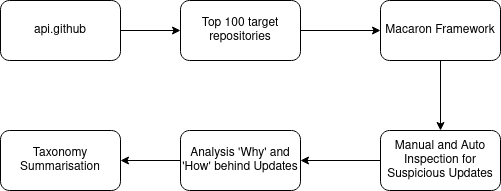
\includegraphics[width=0.7\textwidth]{./screenshot/research_method.png}
\end{center}

\subsection{Data}
We use the self-defined script to fetch the URLs of the top 100 Python and Java repositories from GitHub.
The URLs will then be fed into the Macaron framework to collect the potential suspicious repositories.
We assume that most of the target repositories will not follow the requirements defined in SLSA.
Afterwards, we will pass the suspicious pull requests to the automation scanner.
Then, we will adopt the automation scanner to scan those repositories.

\subsection{Metrics}
To quantify the false positive, we decide to use the \textbf{precision} concept, which is defined as follows.
\[
    \text{Precision} = \frac{TP}{TP + FP}
\]
Also, time spending is of significance. Therefore, we will consider time-consuming, and the severity of the malicious code 
referring to CVE. Finally, we introduce the security metric as follows. The metric will be implemented to compare our framework
to another static scanner. 


\begin{equation}
    SM = (W_p \cdot P) * (W_{tf} \cdot TF) * (\frac{W_{tc}}{TC}) * (W_s \cdot S)
    \end{equation}
    
Where:
\begin{align*}
SM & = \text{Security Scanner Metric} \\
P & = \text{Precision (as a decimal)} \\
W_p & = \text{Weight for Precision} \\
TF & = \text{Total Findings (TP + FP)} \\
W_{tf} & = \text{Weight for Total Findings} \\
TC & = \text{Time Cost} \\
W_{tc} & = \text{Weight for Time Cost} \\
S & = \text{Normalized Severity Score} \\
W_s & = \text{Weight for Severity}
\end{align*}

\subsection{Research Aims}
This research is aim to contribute the Macaron framework, then examine top 100 Python and Java Git 
repositories with this framework. The statistical findings will be further concluded through the further process.
Also, the results will provide the developers and maintainers with a good understanding 
of the vulnerabilities existed in their CI/CD pipelines configuration. Furthermore, the reason behind
these unsafe update will be deeply investigated.

\subsection{Research Objectives}
\begin{enumerate}
    \item \emph{First step: Fetch the repositories build from Python and Java with the top 100 most stars.}
    \item \emph{Second step: Input the repositories name into the Macaron framework to analysis.}
    \item \emph{Third step: Summarize the outputs generated by Macaron and visualize the results with graphs.}
    
    On this step, we will collect the outputs generated from Macaron and to present statistical frequency of vulnerabilities across various CI/CD stages with graph.
    Through viewing the graph, it will be more understandable for what is the popular attack surface in the famous repositories. 
    \item \emph{Fourth step: Manually and automatically inspecting the code base from the potentially problematic repositories 
    due to not comply with the requirements from the SLSA.}
    
    On this step, we are going to incorporate automation tools, like \textbf{Bandit} for Python repositories and \textbf{Find Security Bugs} for Java related repositories.
    Even though automation tools will sometimes generate false positive/negative results, it will save much time for our research.
    Manual code review on the input passed by \textbf{Macaron} framework. As shown in Figure~\ref{fig:downstream-scanner}, the figure provide the overview of the  downstream auto-scanner.
    To further investigate the scope of the attack caused by
    the detected code, we will manually inspect to some extent the malicious code impact the down stream consumers.
    For example, in Python, the \textbf{exec} may execute the Python code and directly exfiltrate the user information of the consumers.
    If the code is injected into the workflow, the build process might be modified.


    \item \emph{Fifth step: Document and investigate the reason for this suspicious updates.}
    
    We will use \textbf{taxonomy} approach to classify the aim and possible methods to achieve it. Tree based taxonomy is able to 
    provide a clear view for the developers to understand how to avoid the different attacks. 
    \begin{figure}
        \centering
        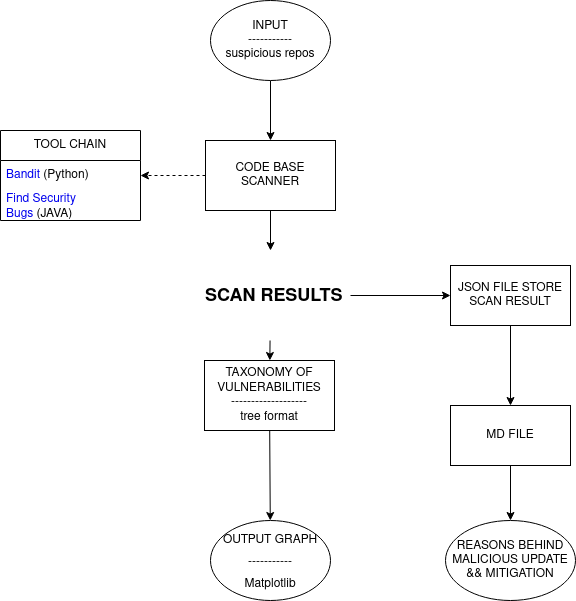
\includegraphics[width=0.7\textwidth]{./screenshot/downstream_scanner.png}
        \caption{Downstream Scanner}
        \label{fig:downstream-scanner}
    \end{figure}
\end{enumerate}

